\let\negmedspace\undefined
\let\negthickspace\undefined
\documentclass[journal]{IEEEtran}
\usepackage[a5paper, margin=10mm, onecolumn]{geometry}
\usepackage{tfrupee}  % Include tfrupee package
\usepackage{gvv-book}
\usepackage{gvv}
\usepackage{cite}
\usepackage{amsmath, amssymb, amsfonts, amsthm}
\usepackage{algorithmic}
\usepackage{graphicx}
\usepackage{textcomp}
\usepackage{xcolor}
\usepackage{txfonts}
\usepackage{listings}
\usepackage{enumitem}
\usepackage{mathtools}
\usepackage{gensymb}
\usepackage{comment}
\usepackage[breaklinks=true]{hyperref}
\usepackage{tkz-euclide}
\usepackage{longtable}
\usepackage{multirow}
\usepackage{hhline}
\usepackage{lscape}
\usepackage{inputenc}  % Automatically handles various encodings

\setlength{\headheight}{1cm}  % Set header height
\setlength{\headsep}{0mm}     % Set header separation
\setlength{\intextsep}{10pt}  % Space between text and floats

\numberwithin{equation}{enumi}
\numberwithin{figure}{enumi}
\renewcommand{\thetable}{\theenumi}

\begin{document}

\bibliographystyle{IEEEtran}
\vspace{3cm}

\title{12.6.5.5.3}
\author{EE24BTECH11020 - Ellanti Rohith}
\maketitle

\renewcommand{\thefigure}{\theenumi}
\renewcommand{\thetable}{\theenumi}


\textbf{Question:}
Find the absolute maximum and minimum value of the function 
\begin{align}
f(x) = 4x - \dfrac{x^2}{2}
\end{align}
in the interval $ \brak{-2, \dfrac{9}{2}} $.



\textbf{Theoretical Solution:}

Given function,
\begin{align}
f(x) = 4x - \dfrac{x^2}{2}
\end{align}

1. First derivative:
\begin{align}
f'(x) = 4 - x
\end{align}

2. Second derivative:
\begin{align}
f''(x) = -1
\end{align}

\subsubsection*{Critical Points:}
To find the critical points, set $ f'(x) = 0 $:
\begin{align}
4 - x = 0 \implies x = 4
\end{align}

\textbf{Nature of Critical Points:}
Since $ f''(x) = -1 < 0 $, $ x = 4 $ is a \textbf{local maximum}.

Evaluate Function at Critical Points and Boundaries:
1. At $ x = -2 $:
\begin{align}
f(-2) = 4(-2) - \dfrac{(-2)^2}{2} = -8 - 2 = -10
\end{align}

2. At $ x = 4 $:
\begin{align}
f(4) = 4(4) - \dfrac{(4)^2}{2} = 16 - 8 = 8
\end{align}

3. At $ x = \dfrac{9}{2} $:
\begin{align}
f\left(\dfrac{9}{2}\right) = 4\left(\dfrac{9}{2}\right) - \dfrac{\left(\dfrac{9}{2}\right)^2}{2} = 18 - \dfrac{81}{8} = \dfrac{144 - 81}{8} = \dfrac{63}{8}
\end{align}

\subsection*{Absolute Maximum and Minimum:}
\begin{itemize}
    \item Absolute Maximum: $ f(4) = 8 $
    \item Absolute Minimum: $ f(-2) = -10 $
\end{itemize}

\textbf{Computational Solution:}

Finding the maximum value of the function can also be done using the Gradient Ascent method:
\begin{align}
x_{n+1} = x_n + \alpha f'(x_n)
\end{align}
Substituting $ f'(x) = 4 - x $:
\begin{align}
x_{n+1} = x_n + \alpha(4 - x_n)
\end{align}

Similarly, the minimum value can be found using the Gradient Descent method:
\begin{align}
x_{n+1} = x_n - \alpha f'(x_n)
\end{align}
Substituting $ f'(x) = 4 - x $:
\begin{align}
x_{n+1} = x_n - \alpha(4 - x_n)
\end{align}


Let $ \alpha = 0.01 $ (learning rate). Then, using numerical iterations:
\begin{align}
x_{min} = -2, \quad f(x_{\text{min}}) = -10
\end{align}
\begin{align}
x_{max} = 4, \quad f(x_{\text{max}}) = 8
\end{align}


The absolute maximum value of the function is $ 8 $ at $ x = 4 $, and the absolute minimum value is $ -10 $ at $ x = -2 $.\\
\textbf{Computational Solution using cvxpy:}
We can find absolute maximum and minimum using $cvxpy$ module in python. Gives $x_{max} = 4, \quad f(x_{\text{max}}) = 8$. However, Python throws an error because the function being minimized is concave. The objective function must be convex for minimization. As a result, we can instead check the endpoints of the boundary within the given interval. At  $ x = -2 $:
\begin{align}
f(-2) = 4(-2) - \dfrac{(-2)^2}{2} = -8 - 2 = -10
\end{align}

At $ x = \dfrac{9}{2} $:
\begin{align}
f\left(\dfrac{9}{2}\right) = 4\left(\dfrac{9}{2}\right) - \dfrac{\left(\dfrac{9}{2}\right)^2}{2} = 18 - \dfrac{81}{8} = \dfrac{144 - 81}{8} = \dfrac{63}{8}\\
f\brak{-2} < f\brak{\frac{9}{2}}
\end{align}

Thus, Minimum occurs at $x=-2$.
\begin{figure}[h]
\centering
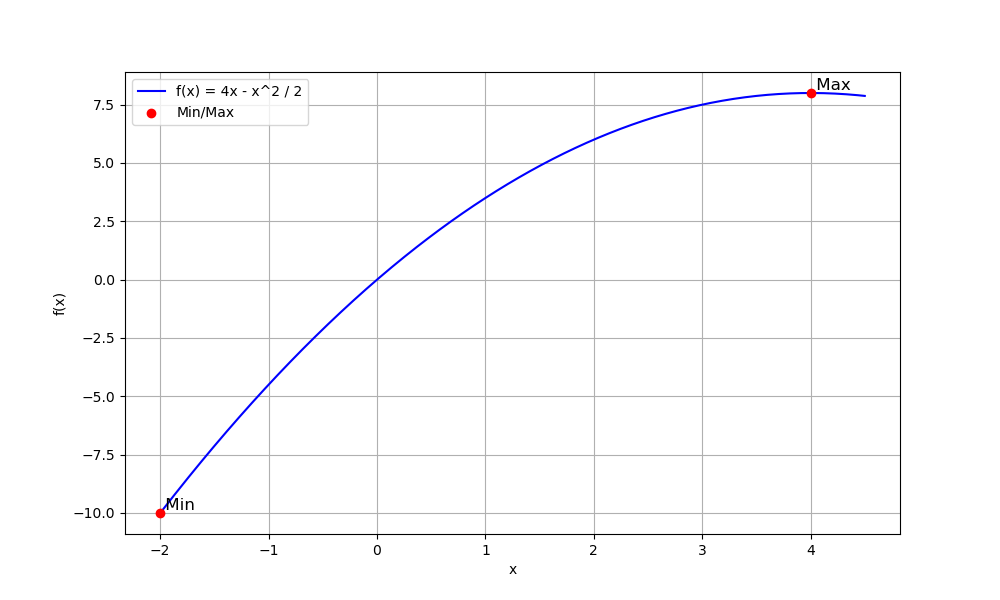
\includegraphics[width=\columnwidth]{Figs/Figure_1.png}
\caption{Plot of the given question.}
\label{fig:Plot1} 
\end{figure}
\end{document}
\end{document}
